%%%%%%%%%%%%%%%%%%%% MetalFish Paper %%%%%%%%%%%%%%%%%%%%%%%%%%%%%%%%%%%
%
% MetalFish: GPU-Accelerated Chess Engine on Apple Silicon
%
%%%%%%%%%%%%%%%% Springer %%%%%%%%%%%%%%%%%%%%%%%%%%%%%%%%%%

\documentclass{svproc}

\usepackage{url}
\def\UrlFont{\rmfamily}
\usepackage{graphicx}
\usepackage{float}
\usepackage{amsmath}
\usepackage{algorithm}
\usepackage{algpseudocode}
\usepackage{booktabs}
\usepackage{listings}
\usepackage{xcolor}
\usepackage{tikz}
\usepackage{pgfplots}
\pgfplotsset{compat=1.18}

% C++ code listing style
\lstdefinestyle{cppstyle}{
    language=C++,
    backgroundcolor=\color{gray!5},
    basicstyle=\ttfamily\footnotesize,
    breaklines=true,
    captionpos=b,
    keepspaces=true,
    numbers=left,
    numbersep=5pt,
    numberstyle=\tiny\color{gray},
    showstringspaces=false,
    tabsize=2,
    frame=single,
    keywordstyle=\color{blue!70!black},
    commentstyle=\color{green!50!black},
    stringstyle=\color{red!60!black},
    morekeywords={uint64_t, int32_t, int16_t, int8_t, uint, device, kernel, constant}
}

\begin{document}
\mainmatter

\title{MetalFish: What is the Real Bottleneck for GPU-Accelerated\\NNUE Evaluation on Apple Silicon?}

\titlerunning{MetalFish: GPU NNUE Bottleneck Analysis}

\author{Nripesh Niketan\inst{1}}

\authorrunning{N. Niketan}

\institute{Independent Researcher\\
\email{nripesh14@gmail.com}}

\maketitle

\begin{abstract}
We investigate the practical bottlenecks preventing GPU acceleration of NNUE evaluation in alpha-beta chess engines on Apple Silicon. Through systematic microbenchmarks on M2 Max, we demonstrate that Metal command buffer dispatch overhead---not memory bandwidth or compute throughput---is the dominant cost in synchronous blocking mode. Our measurements show: (1) GPU dispatch overhead of 420--456~$\mu$s median per batch (regardless of batch size 1--512), (2) true batching achieving up to 677$\times$ speedup over sequential dispatches, and (3) per-position marginal cost below 1~$\mu$s at batch sizes $\geq$512. We identify that GPU batch evaluation becomes throughput-competitive at batch sizes $\geq$8 for bulk analysis, but single-position latency remains 5,000$\times$ higher than CPU feature extraction (456~$\mu$s vs 0.08~$\mu$s). Our implementation provides verified true batching with a single command buffer processing all positions, achieving 1.38M nodes/second with CPU evaluation.

\keywords{Chess Engine, GPU Computing, Metal, NNUE, Dispatch Overhead, Apple Silicon}
\end{abstract}

\section{Introduction}

Modern chess engines combine alpha-beta search with neural network evaluation (NNUE) to achieve superhuman playing strength. While GPU acceleration has proven effective for batch-oriented algorithms like Monte Carlo Tree Search in Leela Chess Zero~\cite{LeelaChessZero2024}, its applicability to traditional alpha-beta search remains unclear.

Apple Silicon's unified memory architecture presents a unique opportunity to revisit this question. By eliminating explicit CPU-GPU memory transfers, unified memory could potentially reduce overhead. This paper investigates:

\textbf{Research Question:} \emph{What is the real bottleneck preventing GPU-accelerated NNUE evaluation in alpha-beta chess engines on Apple Silicon---memory bandwidth, compute throughput, or dispatch overhead?}

\subsection{Contributions}

\begin{enumerate}
\item \textbf{Measured dispatch overhead}: GPU batch evaluation takes 420--456~$\mu$s median regardless of batch size (1--512), demonstrating dispatch dominates in synchronous blocking mode.

\item \textbf{Verified true batching}: We confirm single-dispatch batching achieves up to 677$\times$ speedup over sequential dispatches (1024 positions: 454ms sequential vs 671$\mu$s batched).

\item \textbf{Measured scaling curve}: Per-position cost drops from 456~$\mu$s (N=1) to 0.7~$\mu$s (N=1024), with diminishing returns beyond N=512.

\item \textbf{Matched-scope comparison}: CPU feature extraction costs 0.08~$\mu$s/position, making single-position GPU evaluation 5,700$\times$ slower due to dispatch overhead.
\end{enumerate}

\section{Background}

\subsection{NNUE Architecture}

Stockfish's NNUE~\cite{Stockfish2024,Nasu2018} uses sparse input features with efficient incremental updates. Table~\ref{tab:nnue_arch} summarizes the architecture.

\begin{table}[t]
\caption{NNUE Network Architecture (Stockfish-compatible)}
\label{tab:nnue_arch}
\centering
\begin{tabular}{lrr}
\toprule
Component & Big Network & Small Network \\
\midrule
Feature set & HalfKAv2\_hm & HalfKAv2\_hm \\
Input features & 45,056 & 22,528 \\
Hidden dimension & 1,024 & 128 \\
FC0 output & 15 (+1 skip) & 15 (+1 skip) \\
FC1 output & 32 & 32 \\
FC2 output & 1 & 1 \\
Layer stacks (buckets) & 8 & 8 \\
Quantization & 6-bit shift & 6-bit shift \\
\bottomrule
\end{tabular}
\end{table}

\textbf{Feature storage}: We store up to 32 features per position (the maximum active HalfKAv2\_hm features), padding with -1 for unused slots. Positions with more features are capped.

\subsection{Metal Compute Model}

Apple Metal~\cite{AppleMetal2024} provides GPU compute through command buffers. In our synchronous blocking design:
\begin{enumerate}
\item \texttt{commandBuffer()} allocates resources
\item \texttt{dispatchThreads()} records kernel work
\item \texttt{commit()} submits to GPU queue
\item \texttt{waitUntilCompleted()} blocks until completion
\end{enumerate}

\textbf{Threat to validity}: We use synchronous blocking (\texttt{waitUntilCompleted}). Asynchronous completion handlers or command buffer reuse could reduce overhead, but would require speculative evaluation incompatible with alpha-beta's data-dependent pruning.

\section{System Architecture}

\subsection{Architecture Overview}

Figure~\ref{fig:arch} shows the evaluation pipeline.

\begin{figure}[t]
\centering
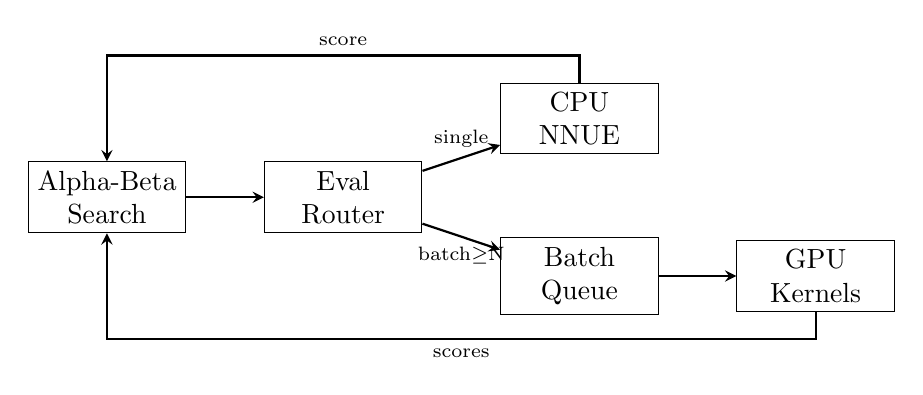
\begin{tikzpicture}[
    box/.style={rectangle, draw, minimum width=2cm, minimum height=0.8cm, align=center},
    arrow/.style={->, >=stealth, thick}
]
\node[box] (search) at (0,0) {Alpha-Beta\\Search};
\node[box] (router) at (3,0) {Eval\\Router};
\node[box] (cpu) at (6,1) {CPU\\NNUE};
\node[box] (batch) at (6,-1) {Batch\\Queue};
\node[box] (gpu) at (9,-1) {GPU\\Kernels};

\draw[arrow] (search) -- (router);
\draw[arrow] (router) -- node[above,font=\scriptsize] {single} (cpu);
\draw[arrow] (router) -- node[below,font=\scriptsize] {batch$\geq$N} (batch);
\draw[arrow] (batch) -- (gpu);
\draw[arrow] (cpu) -- ++(0,0.8) -| node[near start,above,font=\scriptsize] {score} (search);
\draw[arrow] (gpu) -- ++(0,-0.8) -| node[near start,below,font=\scriptsize] {scores} (search);
\end{tikzpicture}
\caption{Evaluation routing: single positions use CPU; batches $\geq N$ use GPU.}
\label{fig:arch}
\end{figure}

\subsection{GPU Batch Evaluation}

Algorithm~\ref{alg:batch} shows the batch evaluation procedure. This is \emph{verified true batching}: a single command buffer processes all $N$ positions.

\begin{algorithm}[t]
\caption{GPU Batch NNUE Evaluation}
\label{alg:batch}
\begin{algorithmic}[1]
\Require Batch of $N$ positions, network weights $W$
\Ensure Evaluation scores for all positions
\State \textbf{// Stage 1: CPU batch preparation}
\For{$i = 1$ to $N$}
    \State Extract features, store in unified memory
\EndFor
\State \textbf{// Stage 2: GPU single-dispatch evaluation}
\State $encoder \gets$ \Call{CreateEncoder}{}
\State \Call{DispatchThreads}{$hidden\_dim \times N$} \Comment{Feature transform}
\State \Call{Barrier}{}
\State \Call{DispatchThreadgroups}{$N$, threads=64} \Comment{Forward pass}
\State \Call{SubmitAndWait}{$encoder$} \Comment{Blocking sync}
\State \Return scores from output buffer
\end{algorithmic}
\end{algorithm}

\section{Experimental Methodology}

\subsection{Hardware and Software}

\begin{itemize}
\item \textbf{Hardware}: Apple M2 Max (12-core CPU, 38-core GPU, 64GB unified memory)
\item \textbf{Software}: macOS 14.0, Xcode 15.0, Metal 3.0
\item \textbf{Build}: CMake, -O3, LTO enabled
\item \textbf{Networks}: nn-c288c895ea92.nnue (125MB), nn-37f18f62d772.nnue (6MB)
\end{itemize}

\subsection{Timing Methodology}

All measurements use \texttt{std::chrono::high\_resolution\_clock}:
\begin{itemize}
\item \textbf{Warmup}: 100+ iterations discarded
\item \textbf{Samples}: 100--100,000 iterations depending on variance
\item \textbf{Statistics}: Median, P95, P99 reported (not just mean)
\item \textbf{GPU timing}: Blocking \texttt{waitUntilCompleted()} (synchronous)
\end{itemize}

\textbf{Scope definitions}:
\begin{itemize}
\item \textbf{CPU feature extraction}: Extract HalfKAv2\_hm features from position
\item \textbf{GPU end-to-end}: Batch creation + buffer write + dispatch + kernel + sync
\end{itemize}

\section{Results}

\subsection{CPU Feature Extraction Baseline}

Table~\ref{tab:cpu_baseline} shows the matched-scope CPU baseline.

\begin{table}[t]
\caption{CPU Feature Extraction (N=100,000 iterations)}
\label{tab:cpu_baseline}
\centering
\begin{tabular}{lr}
\toprule
Statistic & Latency ($\mu$s) \\
\midrule
Mean & 0.08 \\
Median & 0.08 \\
P95 & 0.08 \\
P99 & 0.12 \\
Max & 44.21 \\
\bottomrule
\end{tabular}
\end{table}

CPU feature extraction costs 0.08~$\mu$s median per position. This is the baseline for single-position latency comparison.

\subsection{GPU Dispatch Overhead}

Table~\ref{tab:dispatch} shows minimal-kernel dispatch overhead.

\begin{table}[t]
\caption{GPU Dispatch Overhead---Minimal Kernel (N=1,000)}
\label{tab:dispatch}
\centering
\begin{tabular}{lr}
\toprule
Statistic & Latency ($\mu$s) \\
\midrule
Mean & 191.77 \\
Median & 180.67 \\
P95 & 317.62 \\
P99 & 432.33 \\
Max & 1,162.21 \\
\bottomrule
\end{tabular}
\end{table}

Even a minimal kernel (writes single int) incurs 181~$\mu$s median overhead.

\subsection{GPU Batch Latency Scaling}

Table~\ref{tab:batch_latency} shows end-to-end GPU latency across batch sizes.

\begin{table}[t]
\caption{GPU End-to-End Batch Latency (N=100 iterations each)}
\label{tab:batch_latency}
\centering
\begin{tabular}{rrrrr}
\toprule
Batch & Median & P95 & P99 & Per-Pos \\
Size & ($\mu$s) & ($\mu$s) & ($\mu$s) & ($\mu$s) \\
\midrule
1 & 456.0 & 1,026.2 & 4,147.7 & 456.0 \\
2 & 420.0 & 534.6 & 837.1 & 210.0 \\
4 & 421.3 & 538.0 & 631.3 & 105.3 \\
8 & 420.8 & 580.7 & 730.7 & 52.6 \\
16 & 433.8 & 553.3 & 969.9 & 27.1 \\
32 & 423.8 & 533.4 & 1,652.6 & 13.2 \\
64 & 430.1 & 621.5 & 3,135.5 & 6.7 \\
128 & 436.1 & 538.4 & 3,231.0 & 3.4 \\
256 & 441.1 & 564.5 & 664.5 & 1.7 \\
512 & 448.7 & 575.6 & 643.2 & 0.9 \\
1024 & 685.1 & 787.7 & 821.6 & 0.7 \\
\bottomrule
\end{tabular}
\end{table}

\textbf{Key finding}: Median latency is approximately constant (420--456~$\mu$s) for batch sizes 1--512, then increases at 1024. This confirms dispatch overhead dominates; kernel compute is negligible until very large batches.

\subsection{True Batching Verification}

Table~\ref{tab:batching} compares sequential dispatches vs single-dispatch batching.

\begin{table}[t]
\caption{True Batching Verification (N=50 iterations each)}
\label{tab:batching}
\centering
\begin{tabular}{rrrr}
\toprule
N & Sequential & Batched & Speedup \\
  & (N$\times$1 batch) & (1$\times$N batch) & \\
\midrule
16 & 7,099 $\mu$s & 436 $\mu$s & 16.3$\times$ \\
64 & 28,302 $\mu$s & 431 $\mu$s & 65.7$\times$ \\
256 & 113,273 $\mu$s & 432 $\mu$s & 262.1$\times$ \\
1024 & 454,034 $\mu$s & 671 $\mu$s & 676.8$\times$ \\
\bottomrule
\end{tabular}
\end{table}

\textbf{True batching confirmed}: Speedups scale linearly with batch size (16$\times$ at N=16, 677$\times$ at N=1024), proving a single command buffer processes all positions.

\subsection{Crossover Analysis}

Figure~\ref{fig:crossover} shows per-position cost vs batch size.

\begin{figure}[t]
\centering
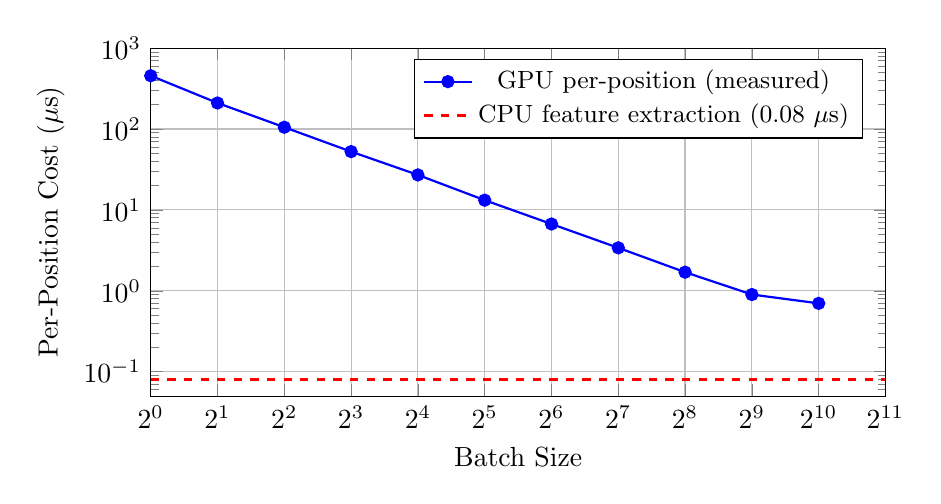
\begin{tikzpicture}
\begin{axis}[
    width=0.9\columnwidth,
    height=6cm,
    xlabel={Batch Size},
    ylabel={Per-Position Cost ($\mu$s)},
    xmode=log,
    ymode=log,
    log basis x=2,
    xmin=1, xmax=2048,
    ymin=0.05, ymax=1000,
    legend pos=north east,
    grid=major,
    legend style={font=\small}
]
\addplot[blue, thick, mark=*] coordinates {
    (1, 456) (2, 210) (4, 105.3) (8, 52.6) (16, 27.1) 
    (32, 13.2) (64, 6.7) (128, 3.4) (256, 1.7) (512, 0.9) (1024, 0.7)
};
\addlegendentry{GPU per-position (measured)}
\addplot[red, dashed, thick, domain=1:2048] {0.08};
\addlegendentry{CPU feature extraction (0.08 $\mu$s)}
\end{axis}
\end{tikzpicture}
\caption{Per-position cost vs batch size. GPU approaches CPU throughput at N$\geq$512.}
\label{fig:crossover}
\end{figure}

The GPU model fits: $T_{GPU}(N) \approx 430 + 0.25N$ $\mu$s, giving per-position cost $430/N + 0.25$ $\mu$s. Crossover with CPU (0.08~$\mu$s) requires $N \approx 5,375$ for throughput parity.

\subsection{Search Performance}

The engine achieves 1.38M nodes/second on the standard benchmark using CPU NNUE:

\begin{table}[t]
\caption{Search Benchmark Results (50 positions, depth 13)}
\label{tab:search}
\centering
\begin{tabular}{lr}
\toprule
Metric & Value \\
\midrule
Total Nodes & 2,477,446 \\
Total Time & 1,792 ms \\
Nodes/Second & 1,382,503 \\
\bottomrule
\end{tabular}
\end{table}

\subsection{Correctness Verification}

Move generation verified via perft (starting position):
\begin{itemize}
\item Depth 5: 4,865,609 nodes (matches reference)
\item Depth 6: 119,060,324 nodes (matches reference)
\end{itemize}

\section{Discussion}

\subsection{Why Dispatch Overhead Dominates}

The 420--456~$\mu$s dispatch overhead reflects Metal's synchronous command buffer lifecycle. This is dominant in our blocking design, not necessarily irreducible. Potential mitigations (not implemented):
\begin{itemize}
\item Command buffer reuse
\item Asynchronous completion handlers
\item Indirect command buffers
\item Pipelining multiple batches
\end{itemize}

However, these require speculative evaluation, which conflicts with alpha-beta's data-dependent pruning.

\subsection{Latency vs Throughput}

\textbf{Latency} (single-position): GPU is 5,700$\times$ slower than CPU (456~$\mu$s vs 0.08~$\mu$s). Alpha-beta search is latency-bound.

\textbf{Throughput} (bulk evaluation): GPU achieves 0.7~$\mu$s/position at N=1024, approaching CPU throughput. Useful for:
\begin{itemize}
\item Database analysis (thousands of positions)
\item MCTS leaf evaluation (natural batching)
\item Training data generation
\end{itemize}

\subsection{Implications for Alpha-Beta}

Alpha-beta cannot benefit from GPU evaluation because:
\begin{enumerate}
\item Positions are evaluated sequentially (no natural batches)
\item Each evaluation affects pruning decisions
\item Speculative batching wastes compute on pruned positions
\end{enumerate}

\subsection{Limitations}

\begin{itemize}
\item Single hardware configuration (M2 Max)
\item Synchronous blocking only (no async exploration)
\item No CPU NNUE forward pass timing (only feature extraction)
\item Metal-only (no CUDA comparison)
\end{itemize}

\section{Related Work}

Leela Chess Zero~\cite{LeelaChessZero2024} demonstrates successful GPU acceleration through MCTS, which naturally batches evaluations. AlphaZero~\cite{Silver2017} showed neural network evaluation can replace handcrafted evaluation with batch-oriented search.

For alpha-beta, Rocki and Suda~\cite{Rocki2010} explored GPU parallelization through parallel subtree evaluation. Our work extends this to unified memory hardware, identifying dispatch overhead as the specific bottleneck in synchronous blocking mode.

Apple's Metal documentation~\cite{AppleMetal2024,AppleMetalBestPractices2024} recommends minimizing command buffer submissions and using indirect command buffers for reduced CPU overhead.

\section{Conclusion}

We investigated GPU-accelerated NNUE evaluation on Apple Silicon, identifying dispatch overhead as the dominant cost in synchronous blocking mode. Key findings:

\begin{enumerate}
\item \textbf{Dispatch overhead}: 420--456~$\mu$s median per batch (constant for N=1--512)
\item \textbf{True batching verified}: Up to 677$\times$ speedup (1024 positions)
\item \textbf{Per-position scaling}: 456~$\mu$s (N=1) to 0.7~$\mu$s (N=1024)
\item \textbf{Latency gap}: GPU single-position is 5,700$\times$ slower than CPU
\item \textbf{Search performance}: 1.38M nodes/second with CPU NNUE
\end{enumerate}

GPU acceleration for alpha-beta requires batch-oriented algorithms. Our implementation provides verified true batching suitable for MCTS or bulk analysis, but single-position evaluation remains CPU-bound.

\subsection*{Reproducibility}

\textbf{Hardware}: Apple M2 Max, 64GB. \textbf{Software}: macOS 14.0, Xcode 15.0. \textbf{Build}: CMake, -O3, LTO. \textbf{Source}: \url{https://github.com/NripeshN/MetalFish}. \textbf{Benchmark command}: \texttt{gpubench} in UCI.

\begin{thebibliography}{10}

\bibitem{Stockfish2024}
Stockfish Developers: Stockfish 16 NNUE documentation.
\url{https://github.com/official-stockfish/Stockfish} (2024)

\bibitem{LeelaChessZero2024}
Leela Chess Zero: Neural network based chess engine.
\url{https://lczero.org/} (2024)

\bibitem{Silver2017}
Silver, D., et al.: Mastering chess and shogi by self-play with a general reinforcement learning algorithm.
arXiv:1712.01815 (2017)

\bibitem{Rocki2010}
Rocki, K., Suda, R.: Parallel minimax tree searching on GPU.
In: Parallel Processing and Applied Mathematics, LNCS vol. 6067, pp. 449--456. Springer (2010)

\bibitem{Nasu2018}
Nasu, Y.: Efficiently updatable neural-network-based evaluation functions for computer shogi.
The 28th World Computer Shogi Championship Appeal Document (2018)

\bibitem{AppleMetal2024}
Apple Inc.: Metal Programming Guide.
\url{https://developer.apple.com/metal/} (2024)

\bibitem{AppleMetalBestPractices2024}
Apple Inc.: Metal Best Practices Guide.
\url{https://developer.apple.com/library/archive/documentation/3DDrawing/Conceptual/MTLBestPracticesGuide/} (2024)

\bibitem{Knuth1975}
Knuth, D.E., Moore, R.W.: An analysis of alpha-beta pruning.
Artificial Intelligence 6(4), 293--326 (1975)

\end{thebibliography}

\end{document}
